\chapter{How does the GA perform on a TSP of a larger scale?}
\section{Introduction}

\par
Considering the characteristics of a Genetic Algorithm, one can assume that they are not the standard method to use on problems of such a small scale as the problem discussed in Chapter 2, since manual or traditional methods can give the solution as well. GAs hold their real value in problems of a larger scale. Here they are capable of giving a feasible solution, where most other methods fail to give one or are just highly inefficient. The constructed GA has proved itself capable of dealing with a simple TSP containing six cities, but how does it perform on a TSP of a larger scale? This chapter will discuss the answer to that question, explaining the obstacles encountered along the way.

\par
The details of the TSP, such as the number of cities and their locations, will be addressed in the next section of this chapter. Then in the third section, the first performance of the GA on this TSP will be discussed. Since the total of possible tours was relatively low for the simple TSP, discussed in the previous chapter, the GA was capable of finding the optimal tour in every run. In this larger TSP however, the number of tours is significantly larger, which meant that the GA did not find the optimal tour in every run. This problem is known as premature convergence and is the topic of the fourth section. In the last section of this chapter a possible method to prevent premature convergence is discussed.

\section{A TSP containing 26 cities}
For this expansion it was decided to extend the problem to 26 cities. To make the problem more realistic, these 26 cities were selected to be located throughout the Netherlands. 

\begin{table} [t]
\parbox{0.4\textwidth}{

\begin{tabular}{l}
1 Amersfoort\\ 
2 Amsterdam\\
3 Apeldoorn\\
4 Arnhem\\
5 Assen\\
6 Breda\\
7 Den Haag\\
8 Den Helder\\
9 Eindhoven\\
10 Emmen\\
11 Enschede\\
12 Groningen\\
13 Haarlem\\
14 Heerenveen\\
15 Heerlen\\
16 ‘s-Hertogenbosch\\
17 Leeuwarden\\
18 Lelystad\\
19 Maastricht\\
20 Middelburg\\
21 Nijmegen\\
22 Rotterdam\\
23 Tilburg\\
24 Utrecht\\
25 Venlo\\
26 Zwolle
\end{tabular}

\label{26cities}
}
\qquad
\begin{minipage}[c]{0.6\textwidth} 
\footnotesize
\centering
\graphicspath{ {Afbeeldingen/} }
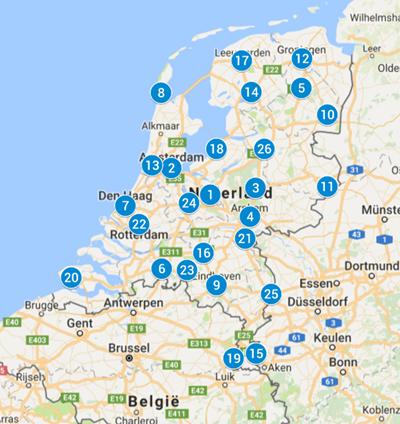
\includegraphics[width=1.2\textwidth, center]{26cities}
\captionof{figure}{26 cities, marked on the map of the Netherlands}
\label{map1}
\end{minipage}
\end{table}

\newpage
\par

The 26 cities are listed in alphabetical order together with a map of the Netherlands (figure \ref{map1}), that marks all of their locations. The objective is thus to find the shortest route that visits all of these cities and returns to the starting point afterwards. The total number of possible tours here is calculated by equation: %future reference needed
\[n = \frac{(26-1)!}{2} =  7.755605e+24\]
This number is significantly larger than the 60 possible tours for the simple TSP, discussed in chapter 2. This is then also the reason why most other methods fail to give a solution or are just inefficient. The manual methods and traditional methods, discussed in the previous chapter, are excellent examples. The Hungarian Algorithm already took 2 hours to perform on a TSP, containing only six cities and even though it did give the optimal solution in the end, it is highly inefficient to apply to this TSP because of the time it would take. In addition, this algorithm is a manual method, which makes it susceptible for human errors. The BIP also fails to give a solution, because the number of integer variables exceeds the limit of the Microsoft Excel linear solver. Even without this limit of variables, a BIP would take a long time to construct, considering all the possible subtours that would have to be added to the program as constraints in order to make sure that the resulting tour meets the criteria, set by the TSP. All of these subtours have to be excluded by manually adding these constraints, which makes the BIP timewise an inefficient method.Therefore it is necessary to turn to other methods, such as Genetic Algorithms. Even though they are not bound to give the optimal solution, they are at least capable of giving a suitable tour that meets the criteria, set by the TSP.

\section{The performance of the GA}

